\section{Tokenizing and Vocabulary}
Next, we tokenize the text data for that we created a custom RegexpTokenizer which tokenizes the text by only allowing words, numbers and some special characters. Even though the dataset is rather cleaned. We choose to keep exclamation marks and question marks as they potentially could add value for sentiment analysis.

Next, we check the top 10 most common words in the dataset. First of all, many stopwords are present in the dataset, these could add some value for sentiment analysis, but we expect them to be more noise than signal. Therefore, we remove the stopwords from the dataset. In addition, many words having similar meanings, e.g. 'feel' and 'feeling' are present, therefore these are also removed by stemming the words.

After text cleaning, we could visualize the common words in the sentences by using a WordCloud, see Figure \ref{fig:wordcloud}.
\begin{figure}[H]
    \vspace*{0.7cm}
    \centering
    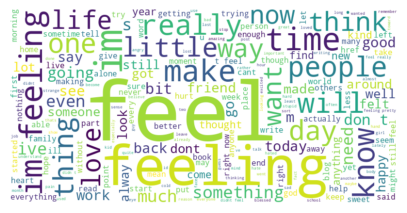
\includegraphics[width=0.4\textwidth]{figures/wordcloud.png}
    \caption{WordCloud of the vocabulary.}
    \label{fig:wordcloud}
    \vspace*{0.7cm}
\end{figure}
As expected many emotional words are present in the vocabulary, e.g. 'love', 'friend', 'hate', 'never', 'go', etc. 

To be able to process the text data, we need to choose a maximum sentence length. A boxplot of the distribution of the lengths of the sequences can be seen in Figure \ref{fig:sequence_length}.
\begin{figure}[H]
    \vspace*{0.7cm}
    \centering
    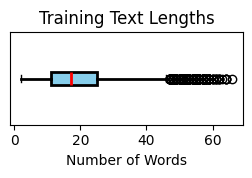
\includegraphics[width=0.22\textwidth]{figures/sentence_length.png}
    \caption{Distribution of the lengths of the sequences.}
    \label{fig:sequence_length}
    \vspace*{0.7cm}
\end{figure}
From the boxplot, we see that the majority of the sequences have a length of around 8 words. We choose to set the maximum sequence length to 10 words. This means that all sequences longer than 10 words are truncated, and all sequences shorter than 23 words are padded with a special token, '<PAD>', to make them all the same length. In addition, we discovered that some sentences are very short, therefore we choose to remove all sentences with a length less than 3 words.

Having our cleaned and tokenized text data, we build a vocabulary from the training dataset. The vocabulary is built by mapping each unique word to an integer. The vocabulary for the training dataset ended up being 10,336 words.

Then, we convert the text data to integers by mapping each word in the text data to the corresponding integer in the vocabulary and pad the sequences to the maximum sequence length. This is done for both the training, validation and test datasets. The text data is now ready to be used for a model.